% !TEX root = /Users/zhuzhuangdi/Desktop/MSUCourses/NaturalLanguageProcessing842/CSE842/FinalReport/latex/final.tex


\section{Evaluation}
We trained and evaluated our sentiment classifier using around 20000 human-labeled tweets, and compare our performance with three baseline sentiment classification approaches.
%
Evaluation shows that our RNN model achieves the highest accuracy compared with baseline models, and has the faster convergence rate compared with models using Convolution Neural Network.
 
\subsection{Available Dataset}\label{subsec:data}
We adopted the Thinknook Dataset\cite{thinknookData} for our evaluation. 
It is composed of tweets from two sources: 
\begin{itemize} 
\item University of Michigan Sentiment Analysis competition on Kaggle\cite{kaggleData}.  
\item Twitter Sentiment Corpus by Niek Sanders\cite{sanderData}.   
\end{itemize} 
%
This dataset contains $1,578,627$ classified tweets since 2012, each row is marked as 1 for positive sentiment and 0 for negative sentiment. 
%
For each sample in the dataset, it contains the tweet ID, the tweet content, and a sentiment label of either \emph{pos} and \emph{neg}. 
%
We extract the tweet content and sentiment labels, and separate the huge dataset into multiple batches of the same size.
%
After preprocessing our data, each batch is a three-dimensional matrix representation which can be used to train and test our RNN model.

\subsection{Baseline Models}
We adopt three baseline approaches to compare with our model: the first two models are based on bag-of-words approaches, that is, these models do not consider the order of words shown in the document, but consider the frequency for a word to appear in the corpus.
\begin{itemize}
\item SVM: For SVM model, we adopt a linear model, and use the Term Frequency - Inverse Document Frequency (TF-IDF) as our input features. TF-IDF is widely used in NLP text classification tasks. It consists of two terms: a term frequency \( tf\) and an inverse document frequency \( idf\):
%\begin{align} 
%tf(t,d) &= 1 + \log(f_{t,d} \\
%idf(t,D) &= log \frac{N}{|\{d \in D: t \in d \}|}
%\end{align}
  
\item Naive Bayes : For naive Bayes model, we use the uni-gram as the input features. Before training model, we adopt the same pre-processing approach as our RNN model.
\item Convolution Neural Network (CNN): We adopt the CNN model for sentiment analysis proposed by Kim \etal \cite{kim2014convolutional}. It applies principals from image processing to a tweet's 2 dimensional sentence vector. In this model, we use a single layer CNN.
\end{itemize}
  


\subsection{ System Implementation} 
%
We used deep learning Python modules called \emph{TensorFlow} \cite{tensorflow} to implement our RNN model. The core parameters are given in Table \ref{fig:rnn_workflow}.
%
The core of the model consists of an LSTM cell that processes one word at a time and computes probabilities of the possible values for the next word in the sentence. 
%
The memory state of the network is initialized with a vector of zeros and gets updated after reading each word. 

\begin{table}[htpb]
\centering
\caption{RNN model parameters}
\label{table:rnn}
\begin{tabular}{|l|l|}
\hline
\textbf{Parameter}      & \textbf{Value} \\ \hline
\textbf{batch\_size}    & 64             \\ \hline
\textbf{embedding size} & 64             \\ \hline
\textbf{hidden layer}   & 50             \\ \hline
\textbf{l2 rate}   & 0.1            \\ \hline 
\textbf{dropout rate}   & 0.5            \\ \hline
\textbf{learning rate}  & 0.0001         \\ \hline
\textbf{max epoch}     & 30             \\ \hline
\end{tabular}
\end{table}

\begin{itemize}
\item \textbf{Truncated Backpropagation.} In order to make the learning process tractable, it is important to create an unrolled version of the network which contains a fixed number of LSTM inputs and outputs, known as the number of steps. The model is then trained on this finite approximation of the RNN. 
%
In our model, we tune the steps to be 30 instead of 140 which is the maximum tweet limit, as most tweets are short and far less than the maximum limit.
%
Then we can perform a backward pass after each such input block.

\item \textbf{Optimizing Loss Function.} We aim to minimize the average negative log probability of the target words: 
\begin{align*}
\text{loss} = -\frac{1}{N} \sum_{i=1}^{N} \ln p_{target_i}
\end{align*}
We implement by using \emph{TensorFlow} 's \emph{seq2seq} library. It will generate the weighted cross-entropy loss for a sequence of logits, based on three inputs: the logits, the targets, and the weights. 

 
\item \textbf{Stacking Multiple LSTMs.} We use multiple layers of LSTMs to process the data so that the output of the current layer will become the input of its succesor.
%
In our model,  we use the libray called \emph{MultiRNNCell} to implement three LSTM networks to strike a balance between the training time and the quality of the model output.
\end{itemize}
 
\subsection{System Comparison}

We use the average accuracy as our metric to evaluate the performance of different models.
%
We explore with different sizes of training data from 5000 tweets to 100000 tweets, and use models trained on different dataset to test coming tweets. 
%
In our experiment, we select a set of 20000 tweets as the testing set.
%
For each set of training data, we use the same pre-processing steps to tokenize tweets.
%
For both RNN and CNN, we use the same word to vector transformations.

\subsubsection{Comparison with traditional models}
Our classification model outperforms SVM and Naive Bayes model by over 20\% accuracy. We use the same set of testing data, and explored with training data of size ranging from 5000 to 100000, and the performance for traditional models cannot reach 80\% even when using the largest size of training data. Figure \ref{fig:acc1} is the results using different size of training data, and Figure \ref{fig:acc2}.
 \begin{figure}[htb]
	\centering
	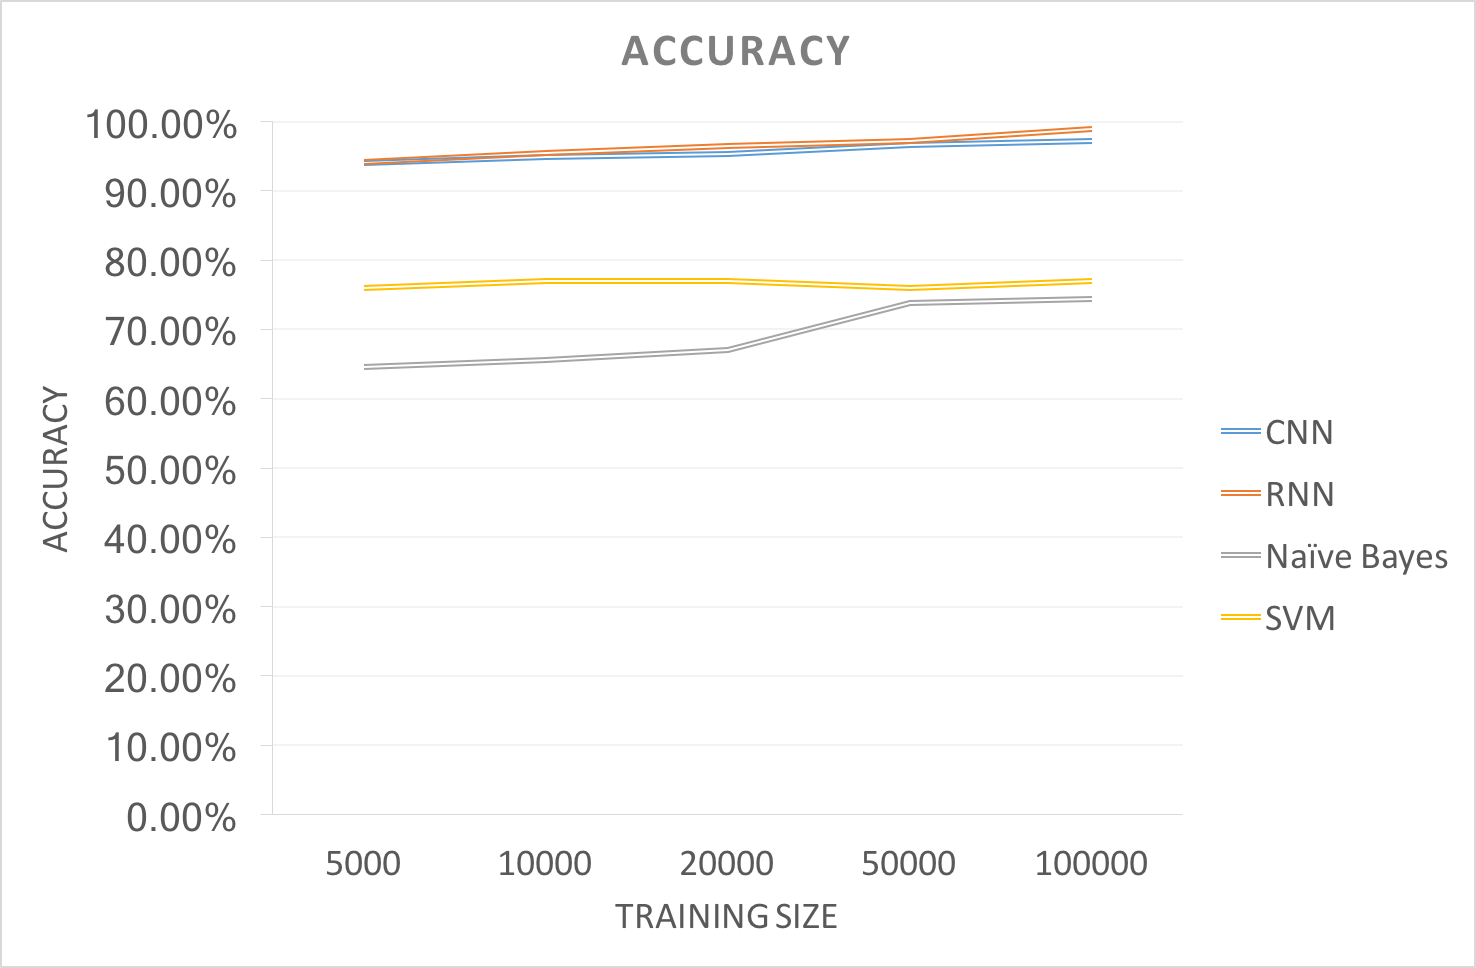
\includegraphics[width=0.9\linewidth]{accuracy1}
	\caption{Model performance with different sizes of training data.}
	\label{fig:acc1}
\end{figure} 
 \begin{figure}[htb]
	\centering
	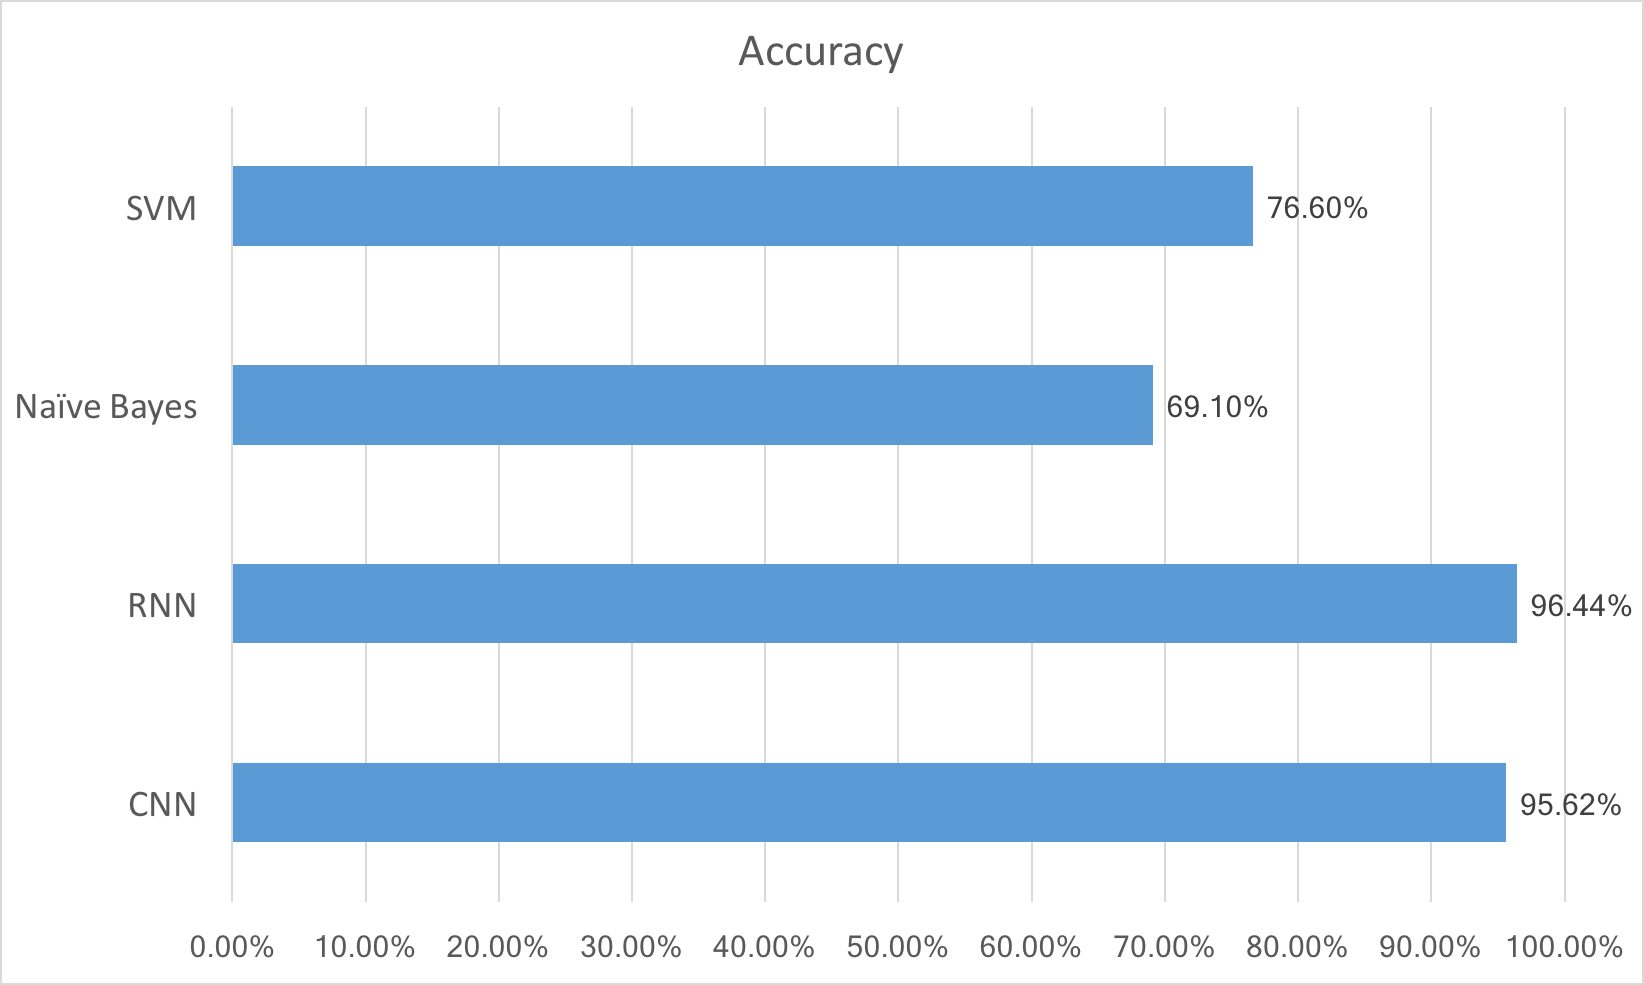
\includegraphics[width=0.9\linewidth]{accuracy2}
	\caption{Average performance}
	\label{fig:acc2}
\end{figure} 

\subsubsection{Comparison with CNN model}
RNN model outperform CNN in terms of accuracy and convergence rate. 
%
We can see from Figure \ref{fig:acc1} that RNN accuracy is larger than CNN.
%
Moreover,  Figure \ref{fig:acc3} shows the accuracy results of training data when in different epoch times. For each epoch (iteration), we feed the RNN and CNN model with a batch of 64 tweets which are mapped to vector representations.
%
We can see that in ,the training accuracy of RNN becomes stable after 12 iterations. But for CNN, it takes more iterations to achieve robustness (after 26 iteration).
% 

 \begin{figure}[htb]
	\centering
	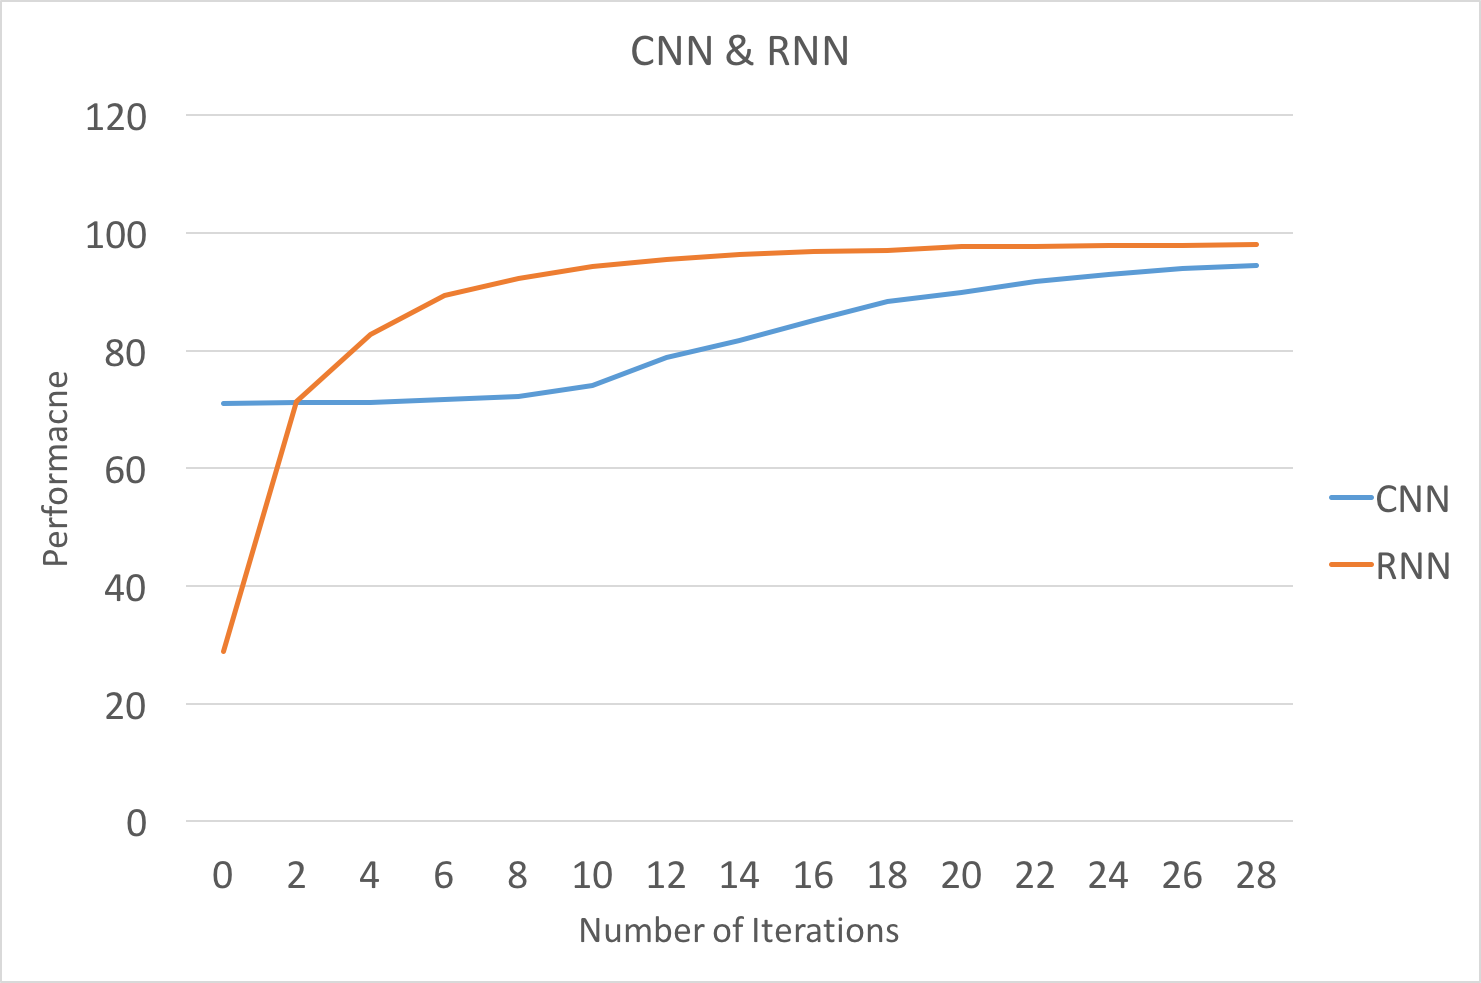
\includegraphics[width=0.9\linewidth]{accuracy3}
	\caption{Convergence rate of RNN and CNN.}
	\label{fig:acc3}
\end{figure} 


 

